\begin{blocksection}
\question
\textbf{2 Chainz}\\
2 Chainz accidentally scrambled his chains! Now there's just one long link that reads "CANHI." Fill in each blank in the code example below so that its environment diagram is the following.

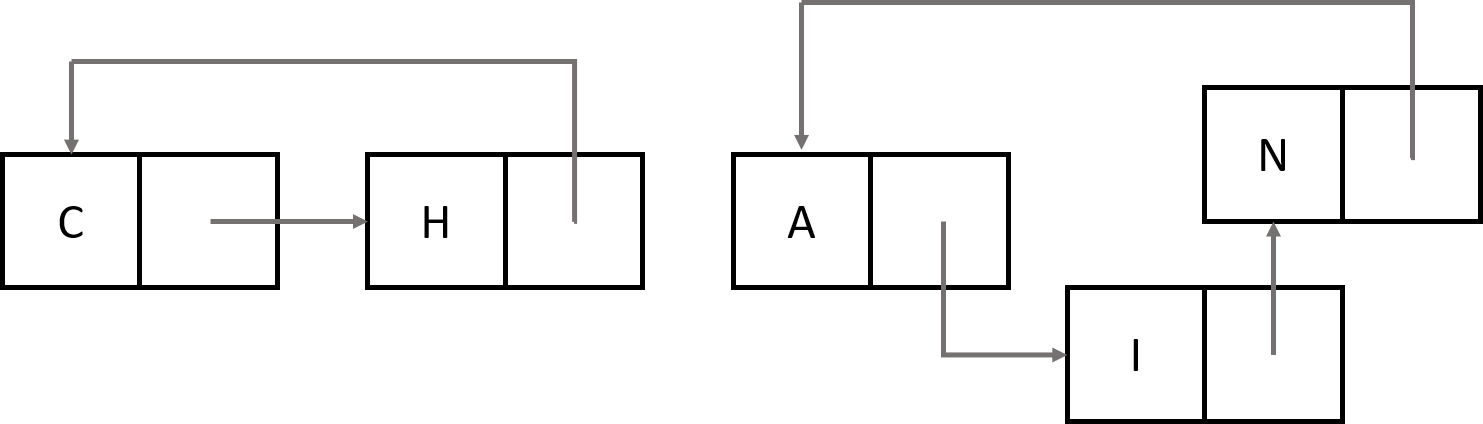
\includegraphics[width=.45\textwidth]{2chainz.png}

\begin{lstlisting}
a = Link("C", Link("A", Link("N", Link("H", Link("I")))))
b = __________________________________________________
a.rest = b.rest.rest
a.___________________________________________ = b.rest
b.rest = _____________________________________________
a.rest.rest = ________________________________________
b.rest.rest.rest = ____________________________________
\end{lstlisting}


\begin{solution}[2in]
\begin{lstlisting}
a = Link("C", Link("A", Link("N", Link("H", Link("I")))))
b = a.rest
a.rest = b.rest.rest
a.rest.rest.rest = b.rest
b.rest = a.rest
a.rest.rest = a
b.rest.rest.rest = b

\end{lstlisting}
\end{solution}
\end{blocksection}

\begin{blocksection}
\begin{guide}
\textbf{Teaching Tips}
\begin{itemize}
	\item The steps can be hard to visualize mentally. Encourage students to draw out a diagram for each step!
	\item Suggest that the general strategy is to reorder each chain and then connect them at the end.
	\item Prod them to think about what happens when we "jump ahead" of a link that we might need later.
\end{itemize}
\end{guide}
\end{blocksection}
